\documentclass[aspectratio=169]{beamer}

\usetheme{Boadilla}
\usefonttheme{professionalfonts}
\setbeamertemplate{navigation symbols}{}
\setbeamertemplate{itemize items}[circle]
\setbeamertemplate{enumerate items}[default]
\setbeamertemplate{headline}{}

\usepackage[utf8]{inputenc}
\usepackage[T1]{fontenc}
\usepackage{lmodern}
\usepackage{amsmath}
\usepackage{booktabs}
\usepackage{tabularx}
\usepackage{array}
\usepackage{hyperref}
\usepackage[strings]{underscore}
\usepackage{listings}
\usepackage{tikz}
\usetikzlibrary{arrows.meta,positioning,fit,calc,shapes.geometric}
\usepackage{xcolor}

\definecolor{courseblue}{HTML}{12355B}
\definecolor{coursegold}{HTML}{C98A2E}
\definecolor{courseice}{HTML}{EEF3F8}
\definecolor{coursegreen}{HTML}{2F6B4F}
\definecolor{coursegray}{HTML}{4B5563}
\definecolor{codebg}{HTML}{F7F9FC}
\definecolor{codecomment}{HTML}{5E6C84}
\definecolor{codestring}{HTML}{0B6E4F}

\setbeamercolor{palette primary}{bg=courseblue,fg=white}
\setbeamercolor{palette secondary}{bg=coursegold,fg=white}
\setbeamercolor{palette tertiary}{bg=courseblue,fg=white}
\setbeamercolor{palette quaternary}{bg=coursegold,fg=white}
\setbeamercolor{structure}{fg=courseblue}
\setbeamercolor{frametitle}{bg=courseice,fg=courseblue}
\setbeamercolor{title}{fg=courseblue}
\setbeamercolor{block title}{bg=courseblue,fg=white}
\setbeamercolor{block body}{bg=courseice,fg=black}
\setbeamercolor{normal text}{fg=black,bg=white}
\setbeamercolor{alerted text}{fg=coursegold}

\setbeamerfont{footline}{size=\scriptsize}

\setbeamertemplate{footline}{
  \leavevmode
  \hbox{
    \begin{beamercolorbox}[wd=.33\paperwidth,ht=2.8ex,dp=1.2ex,leftskip=0.8em]{palette primary}%
      University of Trieste
    \end{beamercolorbox}%
    \begin{beamercolorbox}[wd=.49\paperwidth,ht=2.8ex,dp=1.2ex,center]{palette tertiary}%
      \coursename{} \textbar{} \coursecode
    \end{beamercolorbox}%
    \begin{beamercolorbox}[wd=.18\paperwidth,ht=2.8ex,dp=1.2ex,rightskip=0.8em plus1fil]{palette secondary}%
      \insertframenumber{} / \inserttotalframenumber
    \end{beamercolorbox}%
  }
}

\hypersetup{
  colorlinks=true,
  linkcolor=courseblue,
  urlcolor=coursegreen
}

\lstdefinestyle{coursepython}{
  language=Python,
  basicstyle=\ttfamily\footnotesize,
  keywordstyle=\color{courseblue}\bfseries,
  commentstyle=\color{codecomment}\itshape,
  stringstyle=\color{codestring},
  showstringspaces=false,
  columns=fullflexible,
  keepspaces=true,
  frame=single,
  framerule=0.6pt,
  rulecolor=\color{courseblue},
  backgroundcolor=\color{codebg},
  xleftmargin=0.4em,
  xrightmargin=0.4em,
  aboveskip=0.4em,
  belowskip=0.2em
}

\newcommand{\coursename}{Data-driven Systems Engineering}
\newcommand{\coursecode}{440MI / 305SM}
\newcommand{\coursefooter}{}

\newcommand{\learninggoals}[1]{
  \begin{block}{Learning goals}
  #1
  \end{block}
}

\newcommand{\repoactivity}[1]{
  \begin{block}{Repo activity}
  #1
  \end{block}
}

\newcommand{\readinglist}[1]{
  \begin{block}{Papers and materials}
  {\footnotesize #1}
  \end{block}
}

\newcommand{\coursecontextframe}[5]{
  \begin{frame}{Course Map and Running Cases}
  \centering
  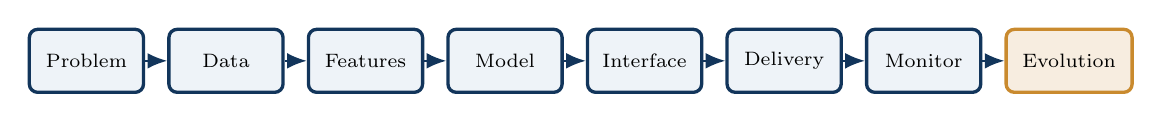
\begin{tikzpicture}[node distance=0.28cm]
  \node[flowbox, minimum width=1.45cm, minimum height=0.8cm] (problem) {\scriptsize Problem};
  \node[flowbox, minimum width=1.45cm, minimum height=0.8cm, right=of problem] (data) {\scriptsize Data};
  \node[flowbox, minimum width=1.45cm, minimum height=0.8cm, right=of data] (features) {\scriptsize Features};
  \node[flowbox, minimum width=1.45cm, minimum height=0.8cm, right=of features] (model) {\scriptsize Model};
  \node[flowbox, minimum width=1.45cm, minimum height=0.8cm, right=of model] (interface) {\scriptsize Interface};
  \node[flowbox, minimum width=1.45cm, minimum height=0.8cm, right=of interface] (delivery) {\scriptsize Delivery};
  \node[flowbox, minimum width=1.45cm, minimum height=0.8cm, right=of delivery] (monitor) {\scriptsize Monitor};
  \node[accentbox, minimum width=1.6cm, minimum height=0.8cm, right=of monitor] (evolution) {\scriptsize Evolution};
  \foreach \a/\b in {problem/data,data/features,features/model,model/interface,interface/delivery,delivery/monitor,monitor/evolution} {
    \draw[arrow] (\a) -- (\b);
  }
  \end{tikzpicture}

  \vspace{0.5em}
  \begin{block}{Today in the course}
  \textbf{Focus:} #1

  \textbf{Bridge:} #2
  \end{block}

  \begin{columns}[T]
  \column{0.48\textwidth}
  \begin{block}{Fraud case}
  {\footnotesize #3}
  \end{block}
  \column{0.48\textwidth}
  \begin{block}{Pasteurization case}
  {\footnotesize #4}
  \end{block}
  \end{columns}

  \vspace{0.3em}
  {\footnotesize \textbf{Course thread:} #5}
  \coursefooter
  \end{frame}
}

\newcommand{\classclosingframe}[4]{
  \begin{frame}{From This Class to the Next}
  \begin{block}{What stays with us}
  #1
  \end{block}

  \begin{columns}[T]
  \column{0.48\textwidth}
  \begin{block}{Project use}
  {\footnotesize #2}
  \end{block}
  \column{0.48\textwidth}
  \begin{block}{Next connection}
  {\footnotesize #3}
  \end{block}
  \end{columns}

  \vspace{0.3em}
  {\footnotesize \textbf{Course thread:} #4}
  \coursefooter
  \end{frame}
}

\tikzset{
  flowbox/.style={
    rounded corners=3pt,
    draw=courseblue,
    fill=courseice,
    very thick,
    minimum width=2.2cm,
    minimum height=0.9cm,
    align=center,
    font=\small
  },
  accentbox/.style={
    rounded corners=3pt,
    draw=coursegold,
    fill=coursegold!15,
    very thick,
    minimum width=2.2cm,
    minimum height=0.9cm,
    align=center,
    font=\small
  },
  arrow/.style={
    -{Latex[length=2.5mm,width=2mm]},
    thick,
    draw=courseblue
  }
}

\usepackage{amssymb}

\title{Class 17: Version Control with Git}
\author{\coursename}
\date{}

\begin{document}

\frame{\titlepage \coursefooter}

\begin{frame}{Agenda}
\begin{itemize}
\item Why version control is required for a growing modeling codebase and a team project.
\item Git fundamentals: commits, history, and differences between versions.
\item Branching and merging, including conflict resolution.
\item Remotes: pushing, pulling, and collaborating through GitHub.
\item Pull requests and code review as a team practice.
\item What must never be committed.
\end{itemize}
\coursefooter
\end{frame}

\begin{frame}{Why version control, and why now}
\begin{itemize}
\item Every previous class produced code that changed over time: notebooks, a Streamlit application, feature pipelines.
\item Without version control, the question ``which version produced this result?'' cannot be answered reliably.
\item Git gives every experiment, threshold choice, and interface change a traceable history; it complements the experiment tracking of Class 19, which records runs but not the code that produced them.
\item The practice must be established now, before the team project (Classes 32--34) makes it indispensable.
\end{itemize}
\coursefooter
\end{frame}

\begin{frame}[fragile]{Git fundamentals}
\begin{lstlisting}[style=coursepython,language=bash]
git init
git clone <url>
git status
git add <file>
git commit -m "message"
git log --oneline
git diff
\end{lstlisting}
\begin{itemize}
\item A commit is a snapshot of the project together with a message, an author, a timestamp, and a reference to its parent commit(s); it is identified by a hash of this content.
\item The commits form a directed acyclic graph: the history. \texttt{git log} traverses it, and \texttt{git diff} shows the difference between two snapshots.
\end{itemize}
\coursefooter
\end{frame}

\begin{frame}{Where a change lives: the four locations}
\centering
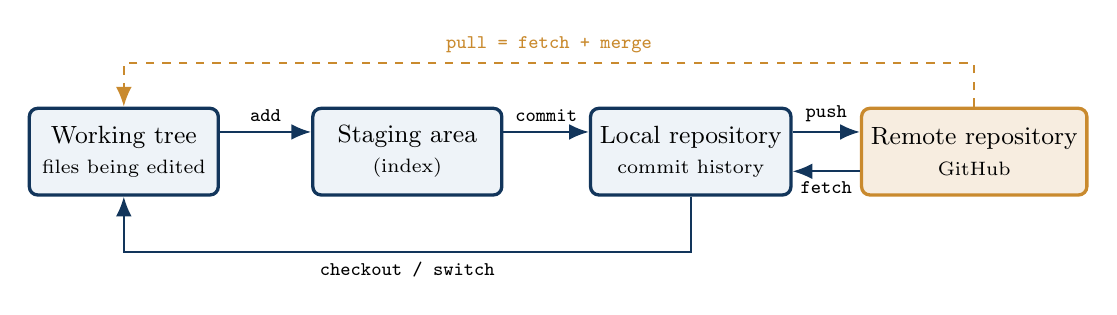
\begin{tikzpicture}[font=\footnotesize, box/.style={flowbox, minimum width=2.4cm, minimum height=1.1cm}]
\node[box] (wt) at (0,0) {Working tree\\\scriptsize files being edited};
\node[box] (ix) at (3.6,0) {Staging area\\\scriptsize (index)};
\node[box] (lr) at (7.2,0) {Local repository\\\scriptsize commit history};
\node[accentbox, minimum width=2.4cm, minimum height=1.1cm] (rr) at (10.8,0) {Remote repository\\\scriptsize GitHub};
\draw[arrow] ([yshift=0.25cm]wt.east) -- node[above, font=\scriptsize\ttfamily] {add} ([yshift=0.25cm]ix.west);
\draw[arrow] ([yshift=0.25cm]ix.east) -- node[above, font=\scriptsize\ttfamily] {commit} ([yshift=0.25cm]lr.west);
\draw[arrow] ([yshift=0.25cm]lr.east) -- node[above, font=\scriptsize\ttfamily] {push} ([yshift=0.25cm]rr.west);
\draw[arrow] ([yshift=-0.25cm]rr.west) -- node[below, font=\scriptsize\ttfamily] {fetch} ([yshift=-0.25cm]lr.east);
\draw[arrow] (lr.south) -- ++(0,-0.7) -| node[pos=0.25, below, font=\scriptsize\ttfamily] {checkout / switch} (wt.south);
\draw[arrow, dashed, coursegold] (rr.north) -- ++(0,0.55) -| node[pos=0.25, above, font=\scriptsize\ttfamily] {pull = fetch + merge} (wt.north);
\end{tikzpicture}
\vspace{0.6em}
\begin{itemize}\footnotesize
\item \texttt{git status} reports the differences between the working tree, the staging area, and the last commit.
\item \texttt{git diff} compares the working tree with the staging area; \texttt{git diff -{}-staged} compares the staging area with the last commit.
\item Only committed changes become part of the history; only pushed commits are visible to the team.
\end{itemize}
\coursefooter
\end{frame}

\begin{frame}{What makes a good commit}
\begin{itemize}\footnotesize
\item \textbf{Atomic:} one logical change per commit. \textbf{Explanatory:} the message states why; the difference already shows what.
\item \textbf{Frequent and consistent:} the history documents the evolution of the project, and each commit leaves the code in a working state where practical.
\end{itemize}
\vspace{0.4em}
\begingroup\footnotesize
\renewcommand{\arraystretch}{1.3}
\begin{tabularx}{\textwidth}{>{\raggedright\arraybackslash}p{3.6cm} >{\raggedright\arraybackslash}X}
\bfseries Uninformative message & \bfseries Informative message \\
\toprule
\texttt{update} & \texttt{Use cost-based threshold (0.06) in fraud app} \\
\texttt{fix} & \texttt{Fit scaler on training split only to avoid leakage} \\
\texttt{final version} & \texttt{Add rolling-mean feature for temperature (w = 10)} \\
\texttt{changes in notebook} & \texttt{Replace label-encoded chi2 by test of independence} \\
\bottomrule
\end{tabularx}
\par\endgroup
\vspace{0.4em}
{\scriptsize Convention: a short summary line in the imperative mood ($\lesssim 50$ characters), optionally followed by a blank line and a body explaining the motivation.\par}
\coursefooter
\end{frame}

\begin{frame}[fragile]{Branching to test an idea safely}
\begin{lstlisting}[style=coursepython,language=bash]
git checkout -b experiment/cost-sensitive-threshold
git add .
git commit -m "Try cost-sensitive threshold tuning"
git push -u origin experiment/cost-sensitive-threshold
# compare results, then merge or discard the branch
\end{lstlisting}
\begin{itemize}
\item A branch is a movable reference to a commit; it isolates an exploratory change, so that \texttt{main} keeps the last validated model and interface.
\item If the experiment does not outperform the baseline, the branch is discarded without affecting \texttt{main}.
\end{itemize}
\coursefooter
\end{frame}

\begin{frame}{Branches and merges as a commit graph}
\centering
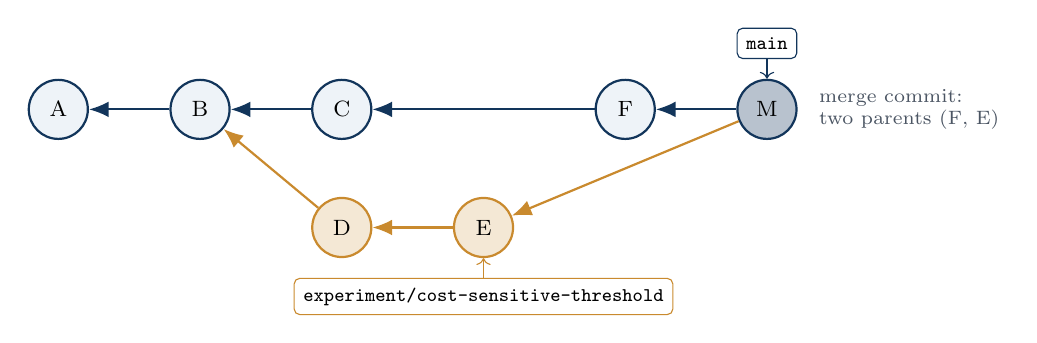
\begin{tikzpicture}[font=\footnotesize, c/.style={circle, draw=courseblue, fill=courseice, thick, minimum size=0.75cm, inner sep=0pt}, e/.style={circle, draw=coursegold, fill=coursegold!20, thick, minimum size=0.75cm, inner sep=0pt}]
\node[c] (a) at (0,0) {A};
\node[c] (b) at (1.8,0) {B};
\node[c] (c) at (3.6,0) {C};
\node[c] (f) at (7.2,0) {F};
\node[e] (d) at (3.6,-1.5) {D};
\node[e] (e) at (5.4,-1.5) {E};
\node[c, fill=courseblue!30] (m) at (9.0,0) {M};
\draw[arrow] (b) -- (a); \draw[arrow] (c) -- (b); \draw[arrow] (f) -- (c);
\draw[arrow, coursegold] (d) -- (b); \draw[arrow, coursegold] (e) -- (d);
\draw[arrow] (m) -- (f); \draw[arrow, coursegold] (m) -- (e);
\node[draw=courseblue, rounded corners=2pt, font=\scriptsize\ttfamily, above=0.25cm of m] (mm) {main};
\draw[->, courseblue] (mm) -- (m);
\node[draw=coursegold, rounded corners=2pt, font=\scriptsize\ttfamily, below=0.25cm of e] (bb) {experiment/cost-sensitive-threshold};
\draw[->, coursegold] (bb) -- (e);
\node[font=\scriptsize, text=coursegray, right=0.15cm of m, align=left] {merge commit:\\two parents (F, E)};
\end{tikzpicture}
\vspace{0.6em}
\begin{itemize}\footnotesize
\item Each commit points to its parent(s); arrows go backwards in time. A branch name is only a reference to the latest commit of that line of work.
\item The experiment branched at B; meanwhile \texttt{main} advanced to C and F. The merge commit M combines both lines and has two parents.
\item Discarding the experiment instead would simply delete the reference \texttt{experiment/\dots}: commits D and E would no longer be reachable from any branch.
\end{itemize}
\coursefooter
\end{frame}

\begin{frame}[fragile]{Merging and conflicts}
\begin{lstlisting}[style=coursepython,language=bash]
git checkout main
git merge experiment/cost-sensitive-threshold
# CONFLICT (content): Merge conflict in scoring.py
\end{lstlisting}
\begin{itemize}
\item A conflict arises when both branches modified the same region of a file. Git marks it with \texttt{<{}<{}<{}<{}<{}<{}<}, \texttt{=======}, and \texttt{>{}>{}>{}>{}>{}>{}>}; resolving it requires a decision about the intended behavior.
\item The resolution consists of choosing or combining the two versions and committing the result, which becomes a merge commit with two parents.
\item Conflicts are an expected part of collaborative development, not an indication of failure.
\end{itemize}
\coursefooter
\end{frame}

\begin{frame}[fragile]{A conflict in practice: the decision threshold}
\begin{columns}[T]
\column{0.5\textwidth}
\textbf{\footnotesize Conflict in \texttt{scoring.py}}
\begin{lstlisting}[style=coursepython]
<<<<<<< HEAD
THRESHOLD = 0.5   # library default
=======
THRESHOLD = 0.06  # cost-based (Class 19)
>>>>>>> experiment/cost-sensitive-threshold
\end{lstlisting}
\textbf{\footnotesize Resolution}
\begin{lstlisting}[style=coursepython]
# c_FN = 100 c_FP; selected on the
# validation split (Class 18)
THRESHOLD = 0.06
\end{lstlisting}
\column{0.48\textwidth}
\begin{itemize}\footnotesize
\item \texttt{HEAD} is the version of the current branch (\texttt{main}); the second block comes from the branch being merged.
\item Git cannot decide which threshold is correct: the choice is a modeling decision, justified by the cost analysis.
\item The resolution removes the markers, documents the reason, and is committed:
\end{itemize}
\vspace{-0.3em}
\begin{lstlisting}[style=coursepython,language=bash]
git add scoring.py
git commit -m "Merge cost-based threshold"
\end{lstlisting}
\end{columns}
\coursefooter
\end{frame}

\begin{frame}[fragile]{Remotes and collaboration through GitHub}
\begin{lstlisting}[style=coursepython,language=bash]
git remote -v
git push origin main
git pull origin main
git fetch
\end{lstlisting}
\begin{itemize}
\item A remote is a shared copy of the repository; in this course, hosted on GitHub.
\item \texttt{push} sends local commits to the remote; \texttt{fetch} retrieves new remote commits; \texttt{pull} performs a fetch followed by a merge into the local branch.
\item Pulling before starting new work limits unnecessary divergence from the rest of the team.
\end{itemize}
\coursefooter
\end{frame}

\begin{frame}{Pull requests and code review}
\begin{itemize}
\item A pull request is a review checkpoint before code reaches a shared branch, where a teammate can detect an unintended change of behavior.
\item Small pull requests can be reviewed thoroughly; large ones tend to be approved without real scrutiny.
\item Review comments address the code and the decisions behind it, not its author.
\item For the team project, a branching convention (e.g.\ one feature branch per task) must be agreed before the first commit, not after the first conflict.
\end{itemize}
\coursefooter
\end{frame}

\begin{frame}[fragile]{What must never be committed}
\begin{lstlisting}[style=coursepython,language=bash]
/.ipynb_checkpoints
/venv
.DS_Store

__pycache__/
*.py[cod]
*.aux
*.log
\end{lstlisting}
\begin{itemize}
\item Excerpt of this repository's \texttt{.gitignore}: environments, caches, and build artifacts are regenerated and need no history.
\item Secrets and credentials must never be committed: a later commit does not remove them from the history, so a leaked credential must be revoked.
\item Large trained artifacts are often better stored outside Git, e.g.\ in a model registry (Class 19).
\end{itemize}
\coursefooter
\end{frame}

\begin{frame}[fragile]{Handling secrets correctly}
\begin{columns}[T]
\column{0.5\textwidth}
\textbf{\footnotesize Incorrect: secret in the code}
\begin{lstlisting}[style=coursepython]
run = neptune.init_run(
    project="team/project",
    api_token="a1b2c3d4...",  # leaked
)
\end{lstlisting}
\textbf{\footnotesize Correct: secret in the environment}
\begin{lstlisting}[style=coursepython]
import os
token = os.environ["NEPTUNE_API_TOKEN"]
run = neptune.init_run(
    project="team/project",
    api_token=token,
)
\end{lstlisting}
\column{0.48\textwidth}
\begin{itemize}\footnotesize
\item The secret is stored outside the repository, e.g.\ exported in the shell or kept in a local \texttt{.env} file listed in \texttt{.gitignore}.
\item The code documents which variable is required, never its value.
\item If a secret has been committed: (1) revoke it immediately, (2) issue a new one, (3) optionally rewrite the history (e.g.\ \texttt{git filter-repo}); once pushed, the secret must be considered compromised regardless of the rewrite.
\end{itemize}
\end{columns}
\coursefooter
\end{frame}

\begin{frame}{Guided practice}
\begingroup\footnotesize
Work in pairs on a shared GitHub repository (about 30 minutes):
\par\endgroup
\vspace{0.3em}
\begin{enumerate}\footnotesize
\item Student A creates the repository with a \texttt{README.md}, a \texttt{.gitignore}, and a file \texttt{scoring.py} containing \texttt{THRESHOLD = 0.5}; student B clones it.
\item Each student creates a branch: A sets \texttt{THRESHOLD = 0.3}, B sets \texttt{THRESHOLD = 0.06}, each with an informative commit message.
\item A pushes and merges first through a pull request reviewed by B.
\item B pulls \texttt{main}, merges it into the own branch, and resolves the resulting conflict, justifying the chosen value in the commit message.
\item B opens a pull request; A reviews it and merges.
\item Both inspect the result with \texttt{git log -{}-oneline -{}-graph} and identify the merge commits.
\end{enumerate}
\vspace{0.3em}
{\scriptsize Deliverable: the URL of the repository; its commit graph must show two branches, one resolved conflict, and two reviewed pull requests.\par}
\coursefooter
\end{frame}

\begin{frame}{Repository connections}
\repoactivity{
\begin{itemize}
\item The commit history and the \texttt{.gitignore} of this repository are a working example of the practices of this class.
\item \texttt{notebooks/}, \texttt{streamlit/}, and \texttt{pasteurization/} contain rapidly changing code that benefits from small, frequent commits.
\item In the team project (Classes 32--34), each team applies these practices to its own shared repository.
\end{itemize}
}
\coursefooter
\end{frame}

\begin{frame}{Papers and materials}
\readinglist{
\fontsize{6.8}{8.2}\selectfont
\begin{columns}[T]
\column{0.5\textwidth}
\begin{itemize}\setlength{\itemsep}{1pt}
\item Chacon, S., Straub, B. (2014). \emph{Pro Git}, 2nd ed. Apress. \href{https://git-scm.com/book/en/v2}{git-scm.com/book}.
\item Driessen, V. (2010). \href{https://nvie.com/posts/a-successful-git-branching-model/}{A successful Git branching model}.
\item Bird, C., Rigby, P.\,C., Barr, E.\,T., Hamilton, D.\,J., German, D.\,M., Devanbu, P. (2009). The promises and perils of mining Git. \emph{Proceedings of the 6th IEEE International Working Conference on Mining Software Repositories}, 1--10.
\end{itemize}
\column{0.5\textwidth}
\begin{itemize}\setlength{\itemsep}{1pt}
\item Bacchelli, A., Bird, C. (2013). Expectations, outcomes, and challenges of modern code review. \emph{Proceedings of the 35th International Conference on Software Engineering (ICSE)}, 712--721.
\item GitHub documentation: \href{https://docs.github.com/en/pull-requests}{pull requests}.
\item Atlassian Git tutorials: \href{https://www.atlassian.com/git/tutorials/using-branches/merge-conflicts}{resolving merge conflicts}.
\end{itemize}
\end{columns}
}
\coursefooter
\end{frame}

\begin{frame}{Take-away message}
\vfill
\centering
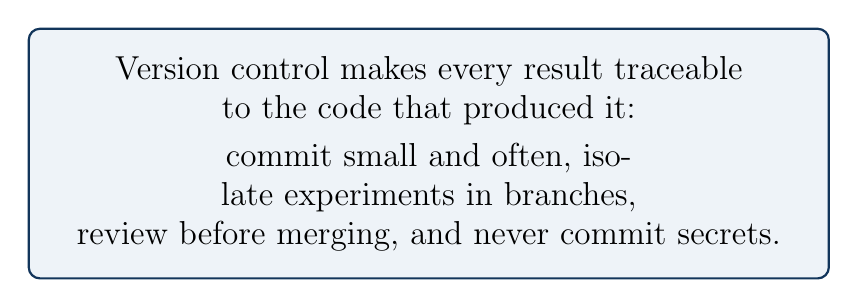
\begin{tikzpicture}
\node[fill=courseice, draw=courseblue, thick, rounded corners=4pt, inner sep=10pt, text width=0.78\textwidth, align=center, font=\large] {Version control makes every result traceable\\ to the code that produced it:\\[0.3em] commit small and often, isolate experiments in branches,\\ review before merging, and never commit secrets.};
\end{tikzpicture}

\vfill
{\Large\bfseries\color{courseblue} Thank you for your attention.}

\vspace{0.4em}
{\small\color{coursegray} Next: Class 18 --- ML modeling.}
\vfill
\coursefooter
\end{frame}

\end{document}
